\let\negmedspace\undefined
\let\negthickspace\undefined
\documentclass[journal]{IEEEtran}
\usepackage[a5paper, margin=10mm, onecolumn]{geometry}
\usepackage{lmodern} % Ensure lmodern is loaded for pdflatex
\usepackage{tfrupee} % Include tfrupee package

\setlength{\headheight}{1cm} % Set the height of the header box
\setlength{\headsep}{0mm}     % Set the distance between the header box and the top of the text

\usepackage{gvv-book}
\usepackage{gvv}
\usepackage{cite}
\usepackage{amsmath,amssymb,amsfonts,amsthm}
\usepackage{algorithmic}
\usepackage{graphicx}
\usepackage{textcomp}
\usepackage{xcolor}
\usepackage{txfonts}
\usepackage{listings}
\usepackage{enumitem}
\usepackage{mathtools}
\usepackage{gensymb}
\usepackage{comment}
\usepackage[breaklinks=true]{hyperref}
\usepackage{tikz}
\usepackage{tkz-euclide} 
\usepackage{listings}
\def\inputGnumericTable{}                                 
\usepackage[latin1]{inputenc}                                
\usepackage{color}                                            
\usepackage{array}                                            
\usepackage{longtable}                                       
\usepackage{calc}                                             
\usepackage{multirow}                                         
\usepackage{hhline}                                           
\usepackage{ifthen}                                           
\usepackage{lscape}
\usetikzlibrary{matrix}

\begin{document}

\bibliographystyle{IEEEtran}
\vspace{3cm}

\title{11.16.3.8.9}
\author{EE24BTECH11002 - Agamjot Singh}
% \maketitle
% \newpage
% \bigskip
{\let\newpage\relax\maketitle}

\renewcommand{\thefigure}{\theenumi}
\renewcommand{\thetable}{\theenumi}
\setlength{\intextsep}{10pt} % Space between text and floats

\textbf{Question:}
\newline
Three coins are tossed at once. Find the probability of getting atmost two tails.
\newline
\textbf{Solution:}
\newline
Sample space $\brak{\Omega}$ is given by,
\begin{align}
    \Omega = \cbrak{HHH, HHT, HTH, HTT, THH, THT, TTH, TTT}
\end{align}
Event space $\brak{\mathcal{F}}$ is given by,
\begin{align}
    \mathcal{F} = 2^{\Omega}
\end{align}
Let $X$ be the random variable,
\begin{align}
    X = \text{number of tails in the sequence}
\end{align}
We express this random variable as a sum of $3$ bernoulli random variables.
\begin{align}
    X = X_1 + X_2 + X_3
\end{align}
where,
\begin{align}
    X_{i} = \begin{cases}
        0 & \quad i^{\text{th}} \text{ toss is a Heads}\\
        1 & \quad i^{\text{th}} \text{ toss is a Tails}
    \end{cases}
\end{align}
$X$ models a binomial distribution.
\newline
For converting to $z$-domain, we use the property,
\begin{align}
    M_{X}\brak{z} = M_{X_1}\brak{z} M_{X_2}\brak{z} M_{X_3}\brak{z}
\end{align}
Extending this system to $m$ tosses, we get, 
\begin{align}
    M_{X}\brak{z} = \prod_{k = 1}^{m} M_{X_{k}}\brak{z}
\end{align}

Let probablity mass function function for the bernoulli random variable $X_{i}$ be given by,
\begin{align}
    P_{X_{i}}\brak{n} = \begin{cases}
        p & \quad n = 0\\
        1 - p & \quad n = 1\\
        0 & \quad n = \mathbb{Z} - \cbrak{0, 1}
    \end{cases}
\end{align}
where $p$ is the probablity of getting heads.
\begin{align}
    M_{X_1}\brak{z} &= \sum_{k = -\infty}^{\infty} P_{X_{1}}\brak{n} z^{-k} = p + \brak{1 - p} z^{-1}\\
    M_{X_2}\brak{z} &= \sum_{k = -\infty}^{\infty} P_{X_{2}}\brak{n} z^{-k} = p + \brak{1 - p} z^{-1}\\
                    &\vdots\\
    M_{X_m}\brak{z} &= \sum_{k = -\infty}^{\infty} P_{X_{m}}\brak{n} z^{-k} = p + \brak{1 - p} z^{-1}\\
    \implies M_{X}\brak{z} &= \brak{p + \brak{1 - p} z^{-1}}^{m}\\
    M_{X}\brak{z} &= \sum_{k = -\infty}^{\infty} \brak{\comb{m}{k} p^{m - k} \brak{1 - p}^{k}} z^{-k}\\
\end{align}
Taking $z$-inverse on both sides, we get,
\begin{align}
    P_{X}\brak{n} = \comb{m}{n} p^{m - n} \brak{1 - p}^{n}
\end{align}
Taking $m = 3$ and $p = \frac{1}{2}$,
\begin{align}
    P_{X}\brak{n} = \comb{3}{n} \brak{\frac{1}{2}}^{3}
\end{align}
Using this probability mass function, the cummulative distribution function C.D.F $\brak{F_{X}\brak{n}}$ is given by,
\begin{align}
    F_{X}\brak{n} = \begin{cases}
        0 & \quad n < 0\\
        \comb{3}{0}\brak{\frac{1}{2}}^3 = \frac{1}{8} & \quad 0 \leq n < 1\\
        \comb{3}{0}\brak{\frac{1}{2}}^3 + \comb{3}{1}\brak{\frac{1}{2}}^3 = \frac{1}{2} & \quad 1 \leq n < 2\\
        \comb{3}{0}\brak{\frac{1}{2}}^3 + \comb{3}{1}\brak{\frac{1}{2}}^3 + \comb{3}{2}\brak{\frac{1}{2}}^3 = \frac{7}{8} & \quad 2 \leq n < 3\\
        \comb{3}{0}\brak{\frac{1}{2}}^3 + \comb{3}{1}\brak{\frac{1}{2}}^3 + \comb{3}{2}\brak{\frac{1}{2}}^3 + \comb{3}{3}\brak{\frac{1}{2}}^3 = 1 & \quad 3 \leq n
    \end{cases}
\end{align}
Let $A$ be an event defined as,
\begin{align}
    A&\colon\text{Getting atmost two tails}\\
    P\brak{A} &= P_{X}\brak{0} + P_{X}\brak{1} + P_{X}\brak{2}\\
              &= \frac{7}{8} = 0.875
\end{align}

\textbf{Simulation}
Running a simulation requires generating random numbers with uniform probability. This is done using OpenSSL's random byte generator.
\begin{enumerate}
    \item $1$ byte of randomly generated uniform data is generated using OpenSSL rand.h.
    \item This random number is scaled down from $\cbrak{0, 1, 2, \dots 255}$ to $\sbrak{0, 1}$ by dividing by 255.
    \item For generating the bernoulli random variable, if this normalized number is less than $p$ then 0 is returned, else 1 is returned.
\end{enumerate}
As number of trials increase, the relative frequency converges to the actual probability of the event.

\begin{figure}[h!]
  \centering
  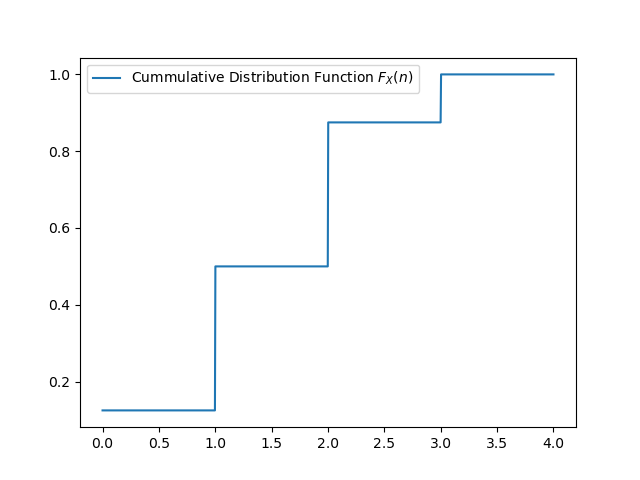
\includegraphics[width=0.7\columnwidth]{figs/cdf.png}
  \caption{CDF Plot}
  \label{label}
\end{figure}

\begin{figure}[h!]
  \centering
  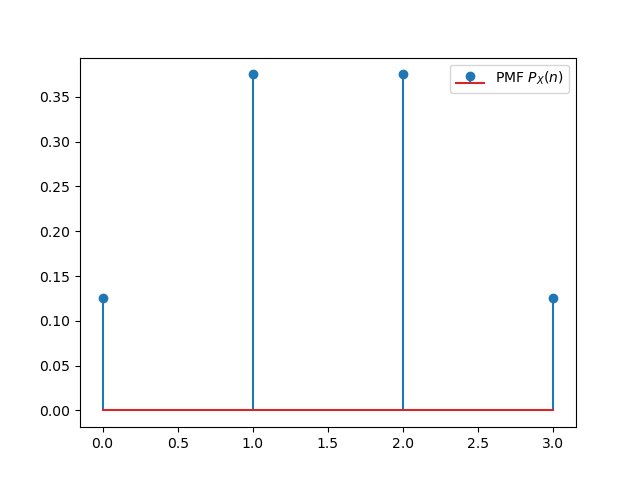
\includegraphics[width=0.7\columnwidth]{figs/pmf1.png}
  \caption{PMF plot for $m$ = 3}
  \label{label}
\end{figure}

\begin{figure}[h!]
  \centering
  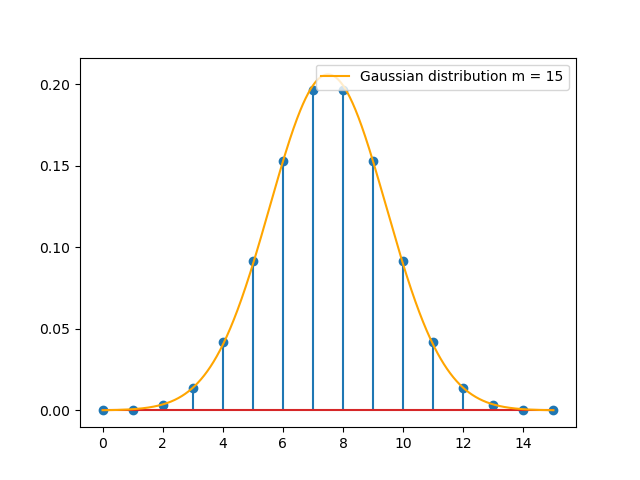
\includegraphics[width=0.7\columnwidth]{figs/pmf2.png}
  \caption{PMF plot for $m$ = 15 with the gaussian distrbution plot}
  \label{label}
\end{figure}

\begin{figure}[h!]
  \centering
  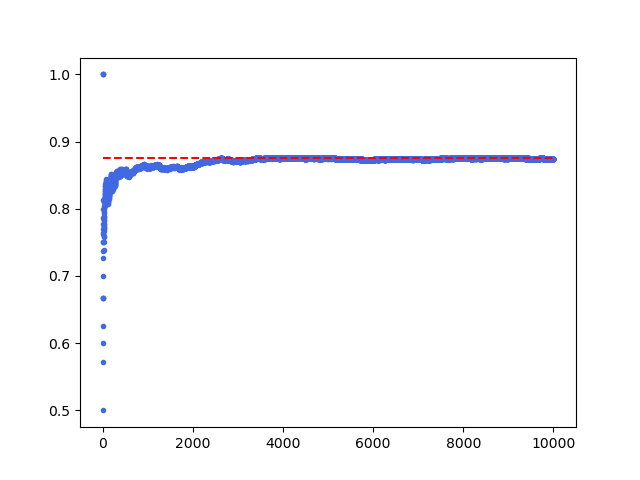
\includegraphics[width=0.7\columnwidth]{figs/sim.png}
  \caption{Relative frequency plot}
  \label{label}
\end{figure}
\end{document}
